%!TEX root = ../main.tex
%%%%%%%%%%%%%%%%%%%%%%%%%%%%%%%%%%
% Links:
%
% Difficulty:
% Companies: 
%%%%%%%%%%%%%%%%%%%%%%%%%%%%%%%%%%

\chapter{Find the majority element}
\label{ch:majority_element}
\section*{Introduction}
It is election time and we are hired to make sure the vote counting is free of mistakes and quick. 
Our job is to determine the winner of this year election. 
Votes are collected as an unordered list and our task is to determine whether there is a clear winner i.e. someone with the majority of the votes (i.e. with more than 50\% of them) or
a new voting session is necessary. 

This problem has been asked at Google and Yahoo interviews for software engineering positions and it is considered medium difficulty. 
Infact, despite the fact it is almost trivial to solve it in linear space, doing so in constant space proves to be quite a bit more challenging and requires non-trivial insights.

As we will see in the coming sections, this problem (and its solution) is a specialization of a more general problem where we need to find out if there is an element in the input list that appears more than $\frac{n}{k}$ times. Clearly, under this definition, we have the majority element problem when $k=2$.
\section{Problem statement}
\begin{exercise}
Given an array $N$ of size $n$, find the majority element i.e. that element that appears more than $\lfloor \frac{n}{2} \rfloor$ times.
If such element does not exists, return $-1$.
	\begin{example}
		\hfill \\
		Given the array $[1,2,3,2,2,1,1,1]$, the function returns $1$ because it appears $4$ times in an array of length $8$.
	
	\end{example}

	\begin{example}
		\hfill \\
		Given the input array $[2, 1, 2]$ the function return $2$ because it is greater than $\frac{3}{2}$.
		
	\end{example}

	\begin{example}
		\hfill \\
		Given the input array $[2, 1, 2,3,4,5]$ the function return $-1$no element appear more than $3$ times.
		
	\end{example}

\end{exercise}

\section{Clarification Questions}

\begin{QandA}
	\item \begin{questionitem} \begin{question} What are the minimum and maximum values an element of the array can take?   \end{question} 	 
    \begin{answered}
		\textit{The minimum and maximum values are $[-10^9, 10^9]$, respectively}.
		This is a good question to ask because if the range is small then we can apply a solution based on bucket counting.
	\end{answered} \end{questionitem}

	\item \begin{questionitem} \begin{question} Can the input array $N$ be modified or shuffled?   \end{question} 	 
    \begin{answered}
		\textit{Yes, the input array can be modified.}
	\end{answered} \end{questionitem}
\end{QandA}

\section{Discussion}
\label{majority_element:sec:discussion}
We will examine three different solutions for this problem. We begin  by looking at the brute-force approach in section \ref{majority_element:sec:bruteforce} Section \ref{majority_element:sec:sorting} will then describe an approach that uses sorting to improve the time complexity of the brute-force approach. Finally,  in section \ref{majority_element:sec:linear} we will examine the optimal approach using the Boyer-Moore algorithm.

\subsection{Brute-force}
\label{majority_element:sec:bruteforce}
The brute force solution is very simple and consist of looping through the array and for each element counting how many times it occurs in the input array. Although this approach is simple, it will not serve you well in an interview scenario as it is far from the optimum and the interviewer is certainly expecting a more sophisticated solution. 
Listing \ref{list:majority_element:bruteforce} shows a possible implementation of this approach. 

\lstinputlisting[language=c++, caption={Sample Caption},label=list:majority_element:bruteforce]{sources/majority_element/majority_element_solution1.cpp}


\subsection{Hash-map approach}
\label{majority_element:sec:hashmap}

A simple improvement on the solution in the section \ref{majority_element:sec:bruteforce} can be made by using a hash-map to store the number of occurrence of each element in the input array. There cannot be more than $n$ different numbers in the the array $N$, thus with a single pass of the input and with a linear cost in space we can calculate the number of occurrence of each element and check if any of the counters at any points gets higher than $\lfloor \frac{n}{2} \rfloor$.

A possible implementation of this approach is shown in Listing \ref{list:majority_element:hashmap}.
The complexity of this approach is $O(n)$ for both space and time. In-fact, even in the worst case  all the elements of the input array are only read and stored once.

\lstinputlisting[language=c++, caption={Solution to the problem of finding the majority element in an array using hash-map.},label=list:majority_element:hashmap]{sources/majority_element/majority_element_solution2.cpp}

\subsection{Sorting - Counting}
\label{majority_element:sec:sorting}
The approach described in section \ref{majority_element:sec:hashmap} is definitely faster then the quadratic brute-force but at a linear price in space. In order not to pay the price in space and to lower the time complexity down from quadratic, we could rely on the fact that in a sorted collection of elements all equal elements appear grouped together e.g. in $[1,1,2,2,3,3,3,4,4,9,9]$, all the $1$s appear at the beginning of the array, followed by all the $2$s, etc. We can then count the number of occurrences of each element in constant space as shown in Listing \ref{list:majority_element:sorting}. The complexity of this approach is bounded by the sorting which costs $O(nlog(n)$ time.

\lstinputlisting[language=c++, caption={Solution  to the problem of finding the majority element in an array using sorting.},label=list:majority_element:sorting]{sources/majority_element/majority_element_solution3.cpp}

\subsection{Sorting - Median}
\label{majority_element:sec:median}
We can, however, make even better use of the fact that we have a sorted collection. The key idea here is that if a majority element exists then this element \textbf{must be the median}. After all, by definition , the median element is right in the middle of the sorted collection. Since the majority element will be occupy \textbf{more} than half of the  positions of the array it must also occupy the median position.
All that is necessary after sorting the array is to check if the median value appears more than $\lfloor \frac{n}{2} \rfloor$ times. 
This idea is implemented in Listing \ref{list:majority_element:median} and has a complexity of $O(nlog(n)$ due to sorting.

\lstinputlisting[language=c++, caption={Linear time constant space solution to the problem of finding the majority element in an array.},label=list:majority_element:median]{sources/majority_element/majority_element_solution4.cpp}

\subsection{Boyer-Moore algorithm}
\label{majority_element:sec:linear}
The best approach to solving this problem in linear time and constant space is, however,  to use the Boyer-Moore algorithm\cite{Boyer1991}.

The algorithm uses two variables to maintain a candidate element $el$ of the sequence and its current count $count=0$ (initialized to $0$). It processes the elements one by one and will perform the following operations:
\begin{itemize}
	\item if we are processing the very first element  of the sequence or \inline{count=0}, it will set $count=1$ and $el$ to that element (this is our first candidate).
	\item otherwise, if the element currently processed is equal to \inline{el}it increments the counter i.e. \inline{count = count+1}
	\item if the element currently processed is different, then it decrements the counter i.e. \inline{count = count -1};
\end{itemize}


At the end of this process the variable \inline{el} will contain a candidate majority element. If the array contains a majority element then \inline{el} \textbf{is} the one. The algorithm correctness can be derived from the fact that the counter will be incremented more times than it will be decremented for the majority element. If we cannot assume that a majority element \textbf{always} exists then a second pass  on the array is necessary in order to count the number of occurrences of \inline{el} in the input array.

Listing \ref{list:majority_element:moore} shows a possible implementation of the Boyer-Moore algorithm. The complexity of this approach is $O(n)$ time and $O(1)$ space because the input array is scanned twice and only two additional integer variables are used.

\lstinputlisting[language=c++, caption={Linear time constant space solution to the problem of finding the majority element in an array.},label=list:majority_element:moore]{sources/majority_element/majority_element_solution5.cpp}




%!TEX root = ../main.tex
%%%%%%%%%%%%%%%%%%%%%%%%%%%%%%%%%%
% Links:
%
% Difficulty:
% Companies: 
%%%%%%%%%%%%%%%%%%%%%%%%%%%%%%%%%%


%\begin{figure}
%	\centering
%	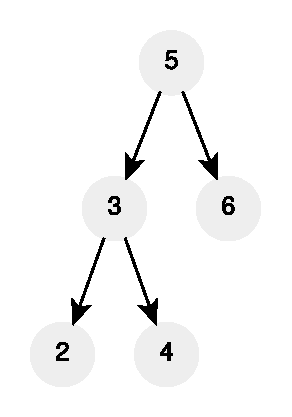
\includegraphics[width=\textwidth]{sources/find_repeated_number_n_divided_3_times/images/example1}
%	\caption[Sample short cpation]{Sample Caption}.
%	\label{fig:find_repeated_number_n_divided_3_times:example1}
%\end{figure}

\section{Find the element repeated $\frac{n}{k}$ times.}
\label{ch:find_repeated_number_n_divided_3_times}
%\section*{Introduction}

\begin{exercise}
\label{example:find_repeated_number_n_divided_3_times:exercice1}
Write a function that, given an array $A$ of $n$ integers and an integer $k$,
returns any of its element that occurs more than  $\frac{n}{k}$.
If such an element does not exists the function returns $-1$.


	%example1
	\begin{example}
		\label{example:find_repeated_number_n_divided_3_times:example1}
		\hfill \\
		Given $A=\{1,2,1,3,1\}$ and $k=3$, the function return $1$ as it occurs $3 > \Big\lfloor\frac{|A|}{3}\Big\rfloor =2$ times.
	\end{example}

	%example2
	%\begin{example}
	%	\label{example:find_repeated_number_n_divided_3_times:example2}
	%	\hfill \\
	%\end{example}
\end{exercise}

%\section{Clarification Questions}
%\begin{QandA}
	%\item 
	%\begin{answered}
		%\textit{}
	%\end{answered}	
%\end{QandA}


\subsection{Boyer-Moore algorithm extended}
\label{find_repeated_number_n_divided_3_times:sec:boyer_moore_extended}
Solution approach:

if you have three distinct elements in the array the solution does not change. You can ignore all three of them.

Therefore, just keep track of the frequencies of two elements.
When you process a new element you can do the following:

1. if you do not have three elements in the frequency list. add it with frequency onesid
2. if the element is equal to another element in the list. increase its frequency
3. if it is a new element (not in the list), decrease the frequency of all in the list by one. Remove any element with frequency zero.
\begin{minipage}{\linewidth}
	\lstinputlisting[language=c++, caption={Sample Caption},label=list:find_repeated_number_n_divided_3_times]{sources/find_repeated_number_n_divided_3_times/find_repeated_number_n_divided_3_times_solution1.cpp}
\end{minipage}

